\documentclass{article}
\usepackage{fancyhdr}
\usepackage{xeCJK}
\usepackage{pifont}
\usepackage{graphicx}
\usepackage{float}
\usepackage{geometry}
\geometry{left=1.5cm,right=1.5cm,top=3cm,bottom=3cm}
%\setmainfont{Times New Roman}  
\setCJKmainfont{Songti SC}
\pagestyle{fancy}
\fancypagestyle{plain}{
    \fancyhf{}
    \fancyfoot[C]{\thepage}
    \renewcommand\headrulewidth{0pt}
}
\begin{document}
    \noindent\textbf{4.2}举例说明何为总线复用?\par
    以Intel8086为例,为了减少总线的引脚数,20位地址总线和16位数据总线时分复用,公用一根总线;一个总线周期里最初的一些时间周期里,总线上传输地址;接下来的周期里传输数据。
    \\[4pt]\par

    \noindent\textbf{4.4}某计算机系统的地址总线宽度是13位,其数据总线宽度是11位,再不采用总线分时复用的情形下,请计算该计算机的最大存储器空间寻址范围。\par
    $2^{13}Bytes=8MB$
    \\[4pt]\par

    \noindent\textbf{4.8}计算机系统什么情况下需要总线仲裁?\par
    多个主设备同时发起对总线的请求时,为了避免总线上请求的冲突,按照预定义的算法确定哪个主设备优先得到总线的使用权。
    \\[4pt]\par

    \noindent\textbf{4.13}异步总线有哪些可能的握手方式?\par
    \ding{172}不互锁方式:主设备发出请求信号,在固定时间间隔D后发出固定长度的读命令;从设备接受信号后,发出固定时间的应答信号,将数据发送到总线上;主设备在读命令后续读取总线上的数据。数据的同步依靠固定的时间间隔来实现。\par
    \ding{173}半互锁方式:主设备发出请求信号,从设备接受信号后,发出固定时间的应答信号,并在数据总线上写入数据;主设备直到接受到从设备应答、接受完总线的数据后才进行撤销请求。\par
    \ding{174}全互锁方式:主设备发出请求信号,从设备接到信号,发出应答和总线数据;主设备接收到应答、读取完数据后撤销请求信号;从设备得知主设备撤销请求后才撤销应答和总线数据。
    \\[4pt]\par

    \noindent\textbf{4.15}周期分裂式总线操作时序有哪些特点?适用于什么样的场景?\par
    这种操作时序将总线周期分为了寻址和数据传送子周期。\par
    将一个耗时长的周期分解为了两个短时间的周期,细化了时间利用的粒度,可以减少总线资源的无效占用,提高总线的利用率,适用于总线请求较多、寻址和数据传输切换较为频繁的场景。
    \\[4pt]\par

    \noindent\textbf{4.19}为什么AMBA总线中没有定义电气特性和机械特性?\par
    AMBA作为一种线上总线标准,其设计独立于处理器芯片的制造工艺;电气特性和机械特性取决于芯片的制造工艺和操作频率,不会体现在AMBA的设计标准中。
    \\[4pt]\par

    \noindent\textbf{4.21}简述AHB总线的流水线机制。\par
    AHB在传输信息时,地址和数据的更新错开;本次的地址更新开始于上次AHB数据传输的最后一个时钟周期,本次的数据更新在下次AHB的传输开始第一个时钟周期被读取。\par
多个AHB中曲奇的地址阶段和数据阶段相互交叠,被称为流水线模式。
    \\[4pt]\par

    \noindent\textbf{4.22}简析AHB中SPLIT操作的优点。\par
    SPLIT操作:流水线操作时因为从机不能及时响应主机,会导致流水线被打断,影响性能。在这种情况下,从机发出SPLIT响应,使得这个请求被挂起,总线的使用权可以被仲裁器让给其他的主机。这样操作可以提高流水线的效率和灵活性,防止因不同步引发的效率损失。
    \\[4pt]\par

    \noindent\textbf{4.23}解释图 4.23中HREADY信号的作用。\par
    图4.23中,突发传输时从机尚未准备好,T2上升沿时HREADY为低,HREADY在T2周期里插入了一个等待周期。在这个等待周期中,所有的信号状态得以保留到下一个周期,等待从机准备好,保证了主机从机操作的同步。
    \\[4pt]\par

    \noindent\textbf{4.25}AHB中突发传输定义了哪些类型?各自有什么特点?\par
    八种类型:\par
    \quad\ding{172}SINGLE\par
    \quad\ding{173}INCR\par
    \quad\ding{174}WRAP4\par
    \quad\ding{175}INCR4\par
    \quad\ding{176}WRAP8\par
    \quad\ding{177}INCR8\par
    \quad\ding{178}WRAP16\par
    \quad\ding{179}INCR16\par
    其中,WRAP模式的传输,传输地址会在最低位进行循环,如WRAP4的其他位不变、低4位在048C上循环;而INCR模式的传输则顺序递增,不会发生循环。
    \\[4pt]\par

    \noindent\textbf{4.30}PCIe 5.0版本中X16的吞吐量63.0 GB/s是如何计算得到的?\par
    单通道PCI-E插槽速度为3938M/s,x16则为16倍于x1的速率为63G/s
    \\[4pt]\par

    \noindent\textbf{4.35}异步串行通信中的起始位和停止位有什么作用?\par
    用于沟通双方区分数据帧的起和止,方便处理收发端之间字符同步的问题。
    \\[4pt]\par

    \noindent\textbf{4.38}什么是I/O端口?一般接口电路中有哪些端口?\par
    IO设备与CPU交互的时候,用一组寄存器来存储需要交互的信息,CPU通过访问这些寄存器来进行和IO设备的交互。这些寄存器被称为IO端口。\par
    数据端口,状态端口,控制端口。
    \\[4pt]\par

    \noindent\textbf{4.40}接口电路的输入需要用缓冲器,而输出需要用锁存器。为什么?\par
    输入时用缓冲器是为了防止外设输入过快,超过处理速度,导致信息拥塞和丢失;\par
    输出使用锁存器是为了可靠地保存输出状态,保证输出信号被接口电路稳定读取。
    \\[4pt]\par

    \noindent\textbf{4.44}分析图 4.68所示菊花链电路,某计算机系统有4个中断源,设计基于菊花链的优先级排队电路(画出电路示意图),并指出优先级最高的是哪个中断源。\par
    见图。设备1的优先级最高。
    \begin{figure}[h]
        \centering
        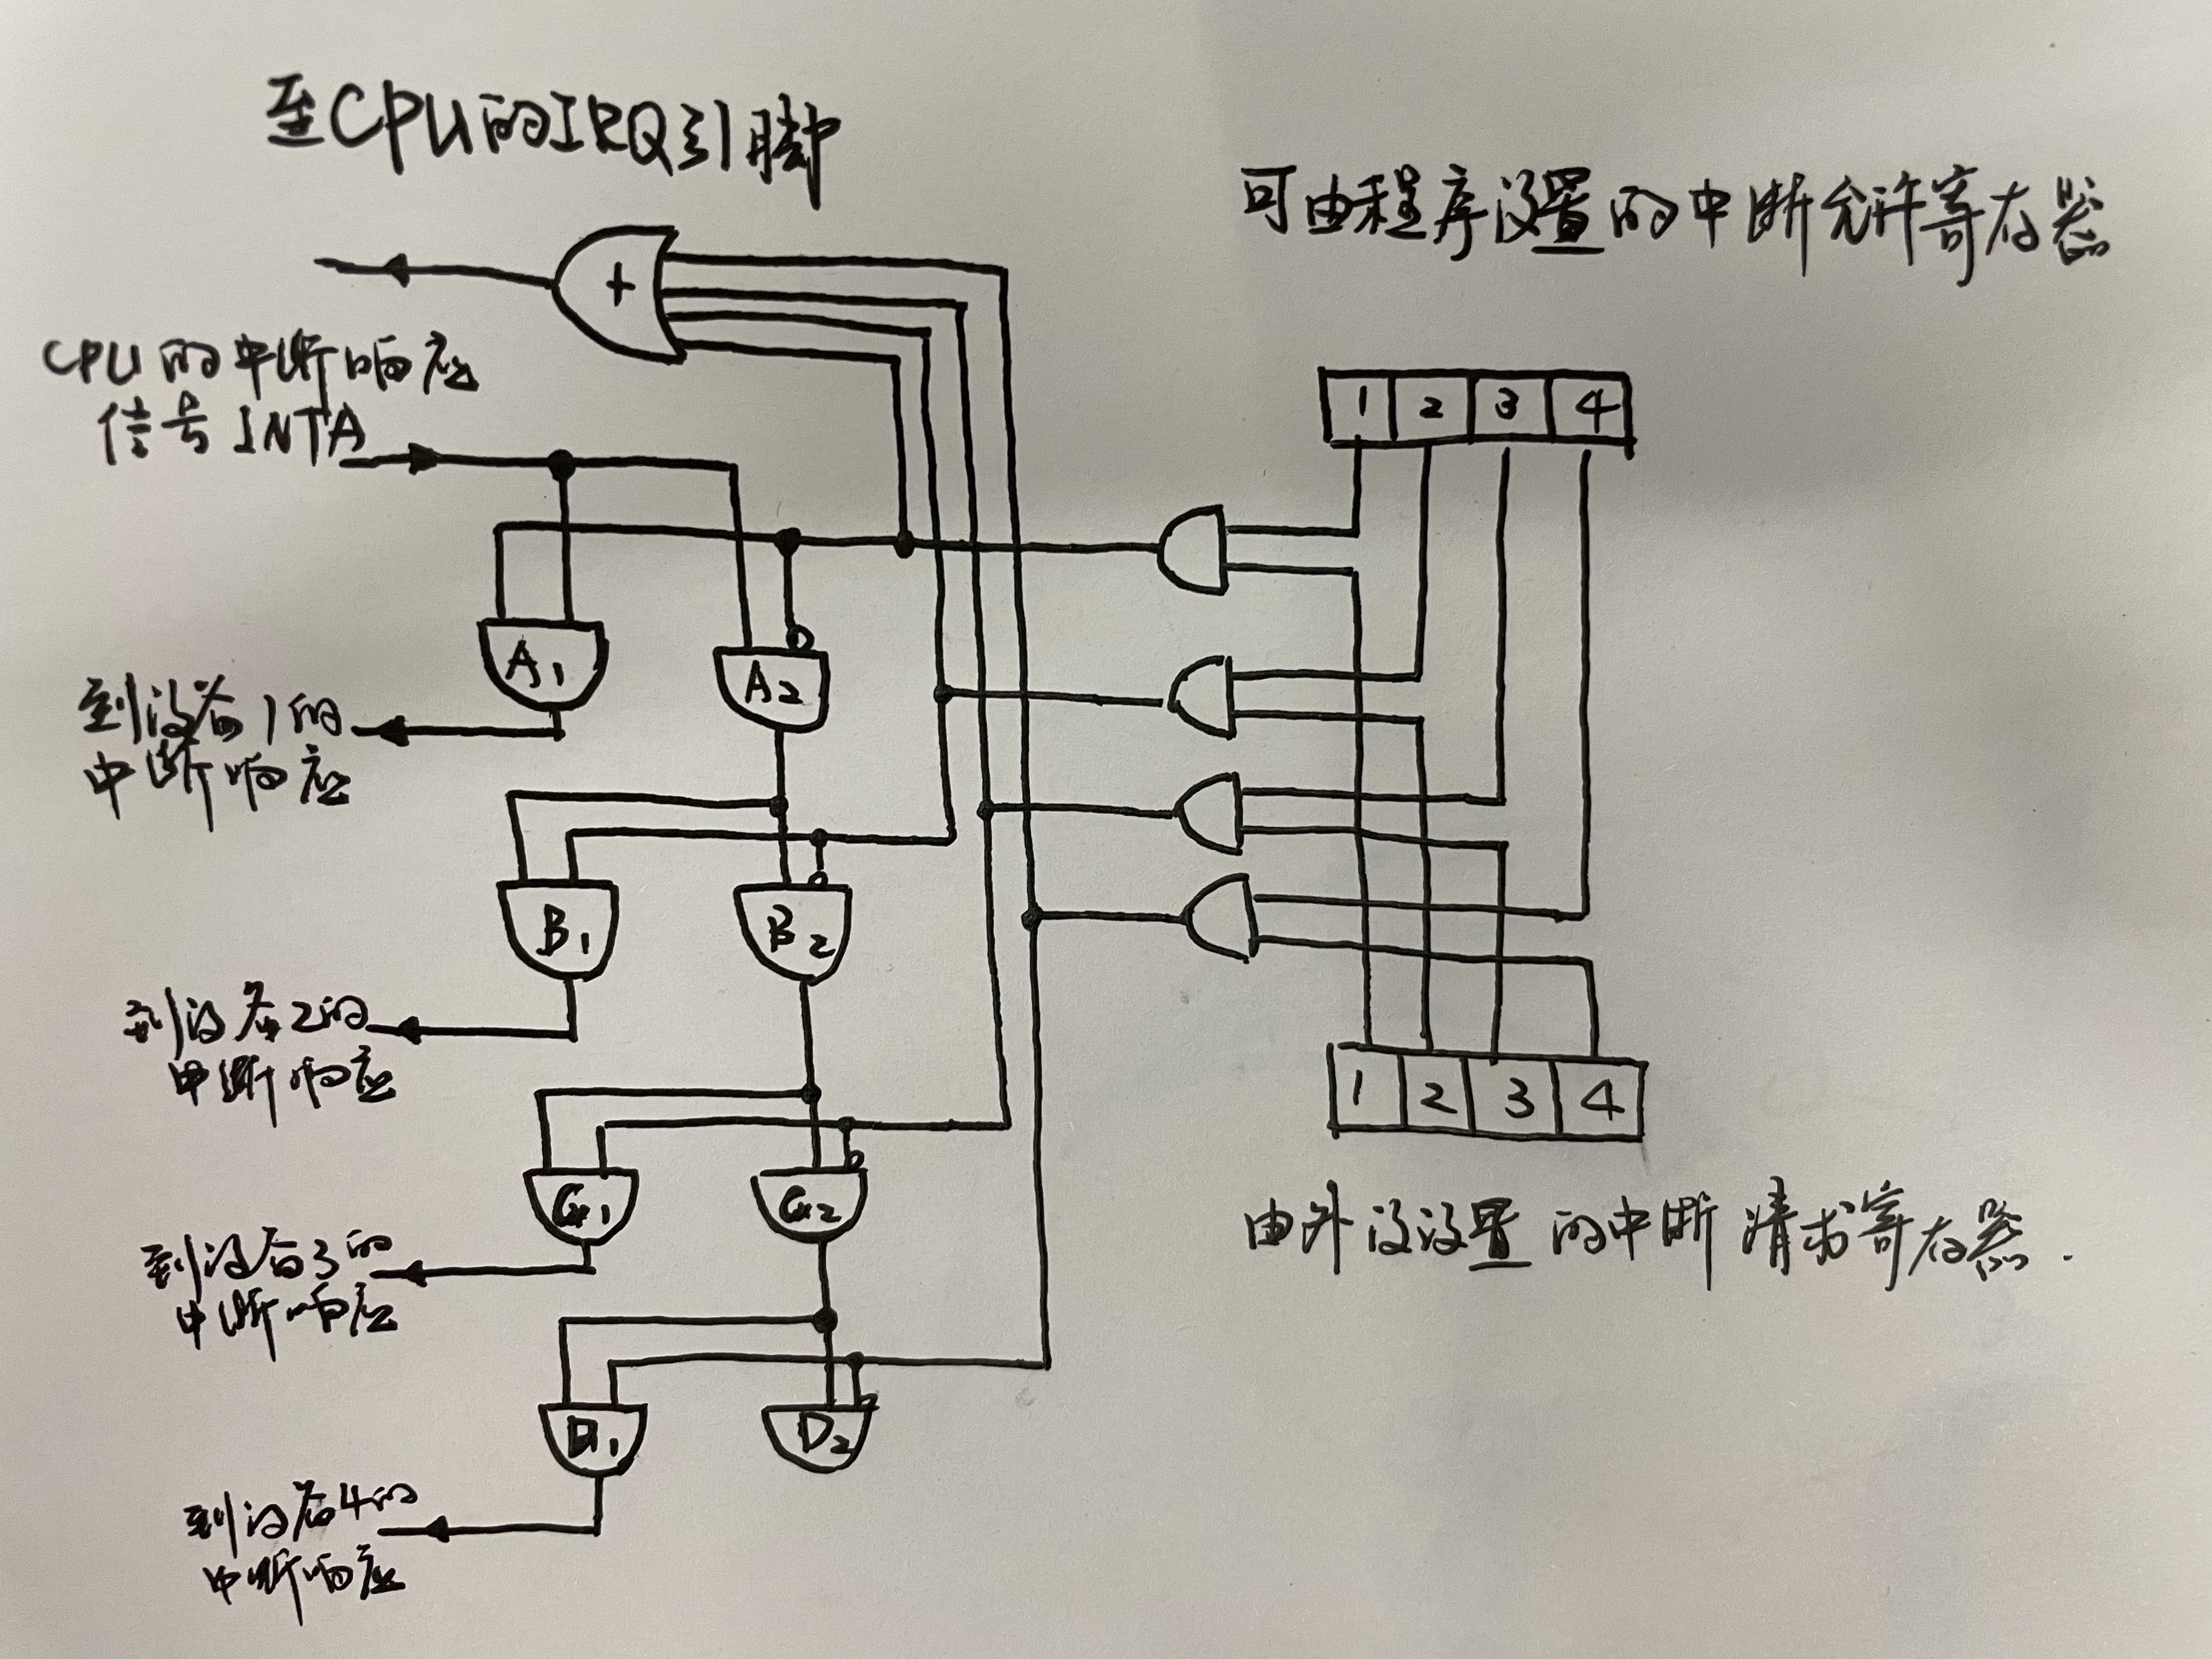
\includegraphics[scale=0.09]{IMG_0909.jpg}
    \end{figure}
    \\[4pt]\par

    \noindent\textbf{4.45}名词解释:中断向量表。\par
    所有中断子程序的入口地址有一块集中的存放区域,称为中断向量表。中断发生时,系统读取中断信号,在中断向量表中查找对应子程序的入口地址,运行中断服务。
    \\[4pt]\par

    \noindent\textbf{4.51}什么是矩阵键盘的行扫描法?\par
    将键盘的键位映射成矩阵,每行每列的交点用电键链接。\par
    每行一端接高电平,另一段接多位输入端口;每列接多位输入端口。
一开始,输出端口向各列输出0;如果输入端口得到的输入为全1,那说明没有任何一个电键按下。\par
    否则,循环在输入端口每一列尝试:该列输出0,其他列输出1,此时看输入端口,如果某一行为0,说明该列该行的电键被按下,以此来定位行列。
    \\[4pt]\par

    \noindent\textbf{4.53}简述LED数码管的动态显示原理。\par
    以共阴极为例,静态显示时,只要选择七段数码管中需要点亮的段输入高电平,其他位输入低电平,com端接低电平即可实现单个七段数码管的点亮。\par
多位七段数码管同时显示数字需要需要动态显示方式,方法是轮流显示每每一位数码管1-2毫秒。所有的数码管共用7位的选段码,在要显示某一位时,输入要点亮该位的选段码,并将该位的com端输入低电平,其他位com端输入高电平,持续1-2ms,然后切换到下一位用下一位的选段码进行同样的操作,以此循环,在观感上就做到了不同位同时显示不同数字。
    \\[4pt]\par

    \noindent\textbf{4.58}异步串行通信系统中,采样数据时为什么要在数据位的中间?\par
    防止收发端在有时钟偏差的情况下,时钟误差进行积累,导致采样数据格式错误,在数据位的中间进行采样防止了在数据位边沿的采样导致采样收到了其他数据位影响。
    \\[4pt]\par

    \noindent\textbf{4.61}描述I2C总线协议中的状态,并画出状态转移图。\par
    \quad\ding{172}总线空闲(I)\par
    \quad\ding{173}启动数据传输(S)\par
    \quad\ding{174}停止数据传输(P)\par
    \quad\ding{175}等待/数据无效(Q)\par
    \quad\ding{176}重新启动(Sr)\par
    \quad\ding{177}数据有效(D)\par
    \quad\ding{178}应答(A)或非应答(N)\par
    见图。
    \begin{figure}[h]
        \centering
        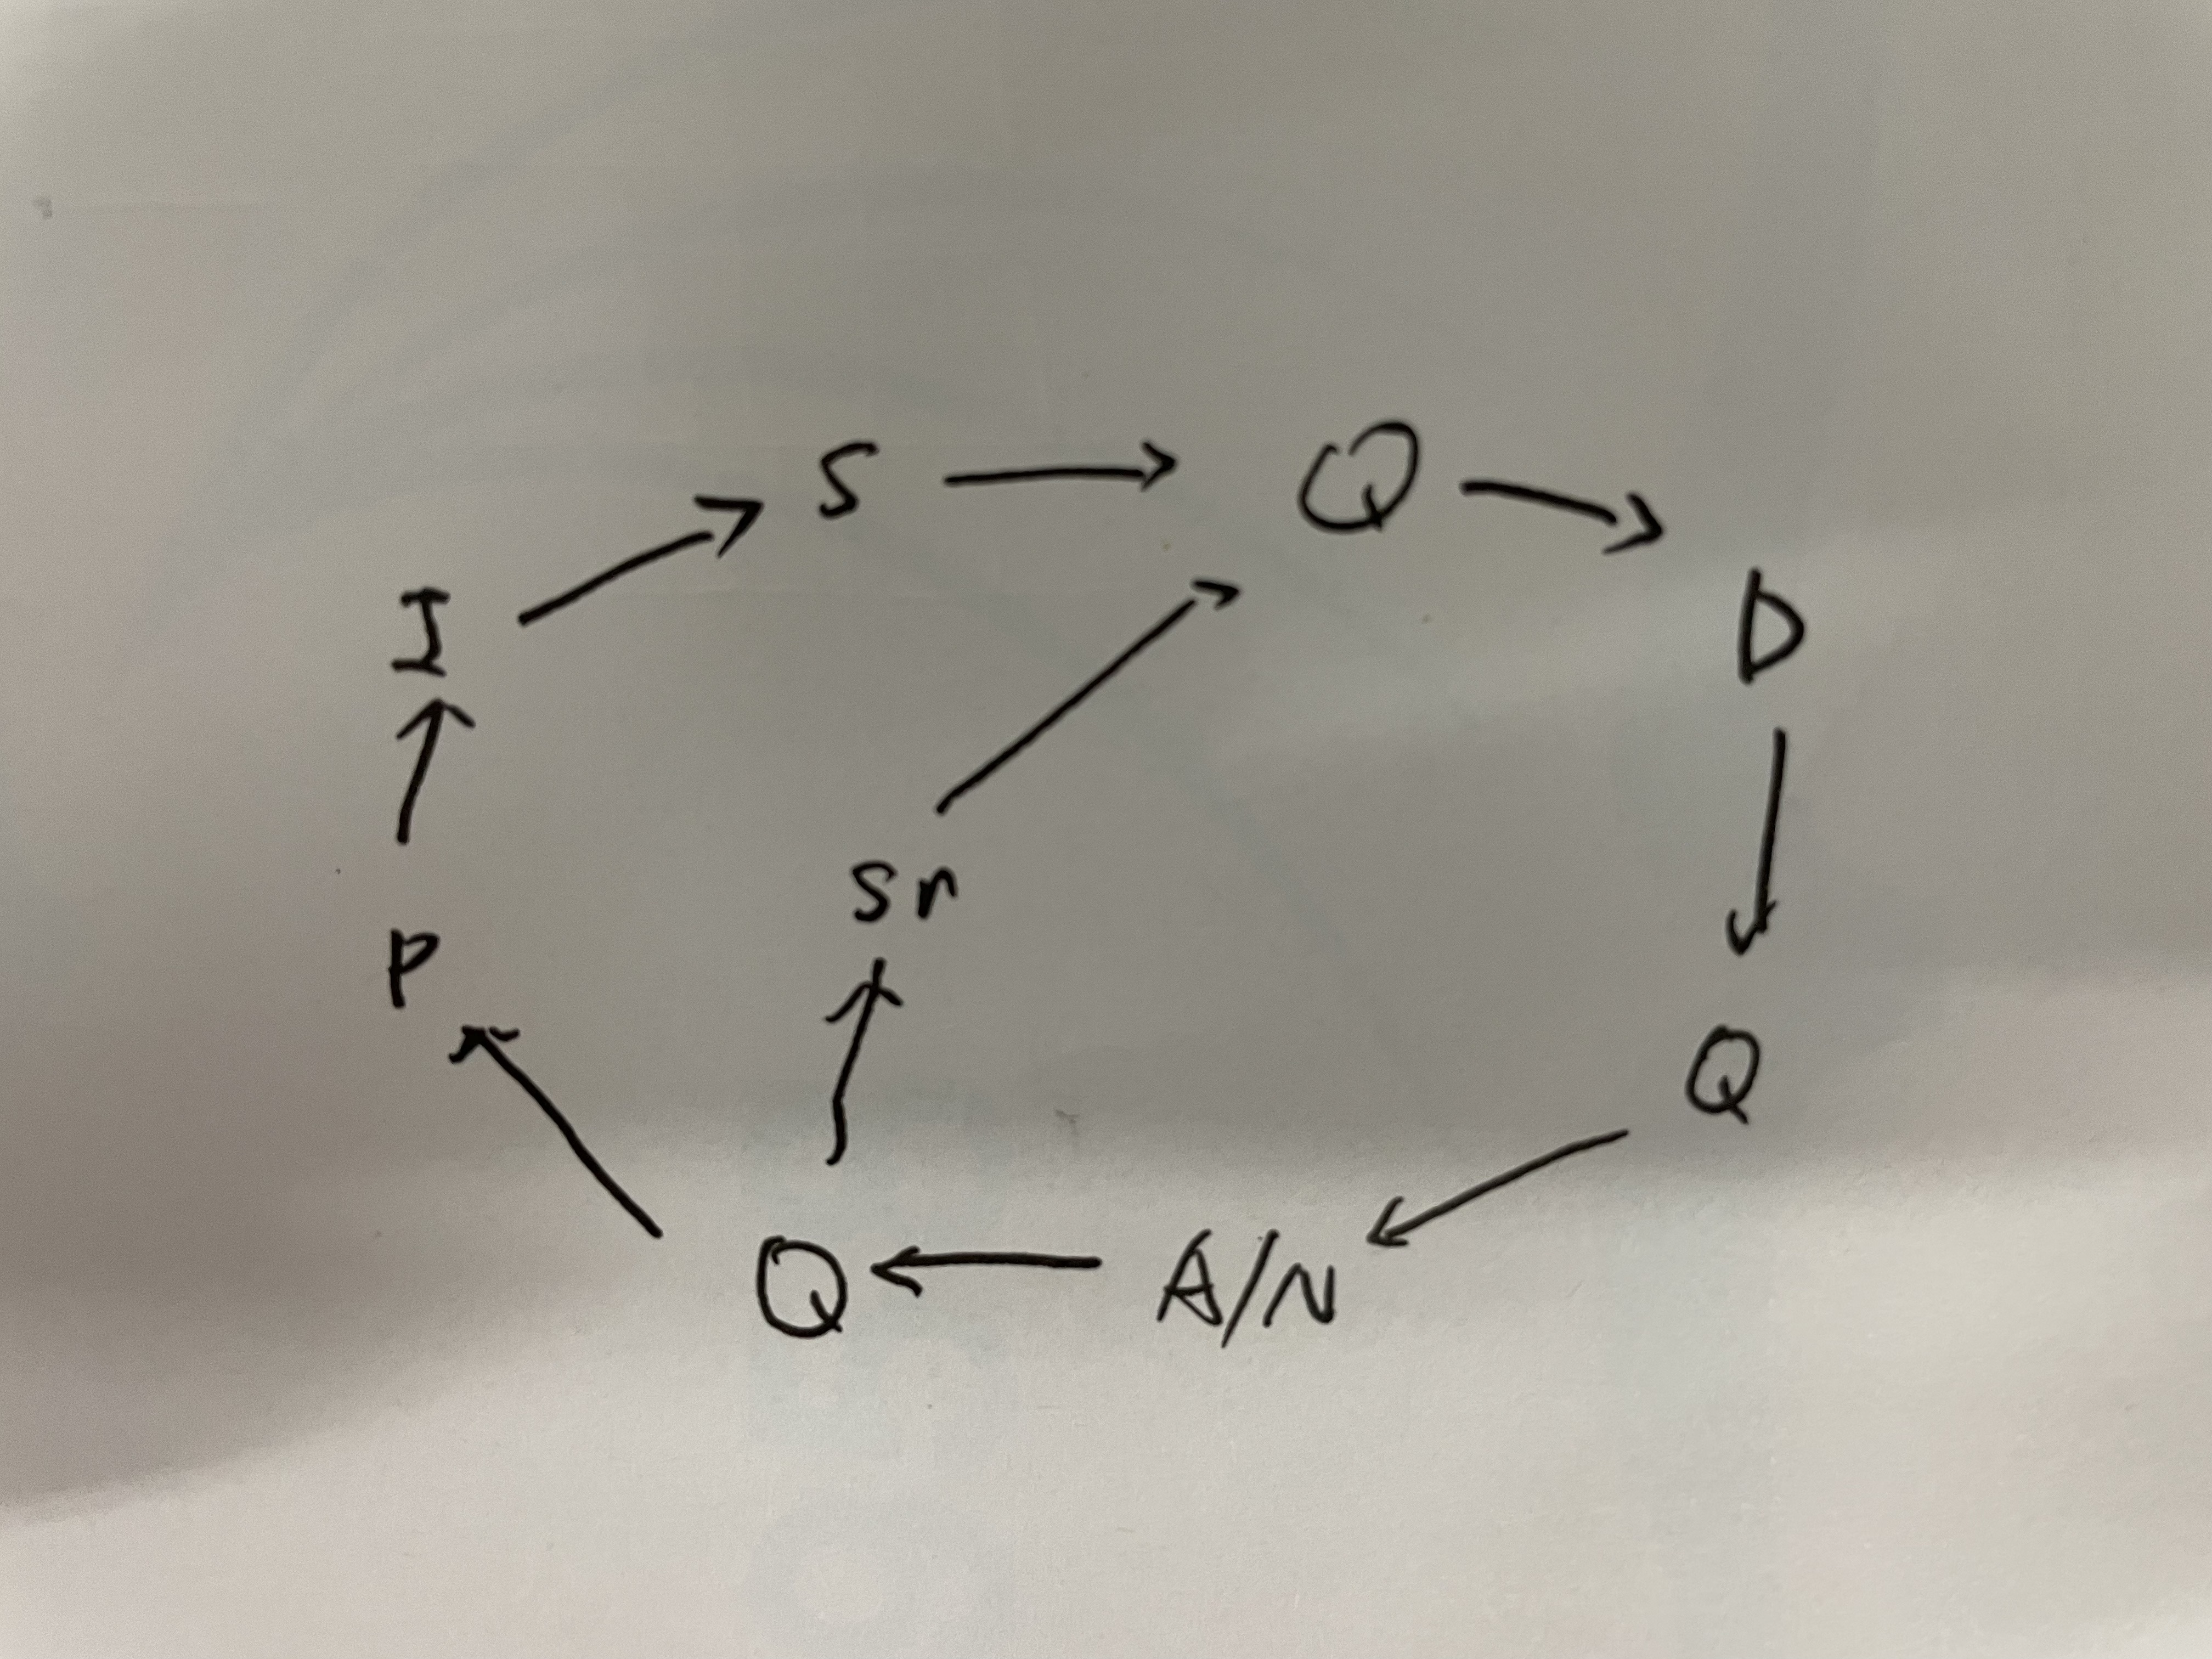
\includegraphics[scale=0.05]{IMG_0910.jpg}
    \end{figure}
    \\[4pt]\par
\end{document}